% !TEX program = xelatex
\documentclass{kaw}

\usepackage[official]{eurosym}
\usepackage[table]{xcolor}
\usepackage{soul}
\usepackage{multicol}
\usepackage{paralist}
\usepackage[para]{footmisc}
\usepackage{graphicx}
\usepackage{mdframed}
\usepackage{wrapfig}
\usepackage{pgfplots}
\usepackage{framed}
\usepackage{caption}
\usepackage{subcaption}
\usepackage{mathtools}
\usepackage{float}
\usepackage{todonotes}
\usepackage{microtype}
\usepackage{pgfplots}
\usepackage{tikz-cd}
\usepackage{tikz}
\usepackage{minted}
\pgfplotsset{scaled y ticks=false, scaled x ticks=false, compat=1.5}
\usetikzlibrary{shapes,arrows,positioning,calc,decorations.pathmorphing,fit}

%%%%%%%%%%%%%%%%%%%%%%%%%%%%%%%%%%%%%%%%%%%%%%%%%%%%%%%%%%%%%%%%%%%%%%%%%%%%%%%%
%% Syntax appearance

\definecolor{darkred}{HTML}{600018}
\definecolor{darkblue}{HTML}{1D2F73}
\definecolor{darkgreen}{HTML}{417505}
\definecolor{lightblue}{HTML}{76E9BB}

\newcommand{\ruleAcc}[1]{\textsc{#1}}
\newcommand{\variable}[1]{{\color{darkblue} \mathtt{ #1 } }}
\renewcommand{\Varid}[1]{{\texttt{#1}}}
\renewcommand{\Conid}[1]{{\texttt{#1}}}

%subst varsym  a = "{\color{darkblue}  \texttt{" a "}}"
%subst numeral a = "{\color{darkgreen} \texttt{" a "}}"
%subst string  a = "{\color{darkgreen} \texttt{\char34" a "\char34}}"

%format family = "\mathbf{family}"
%format forall = "\forall\!"

%%%%%%%%%%%%%%%%%%%%%%%%%%%%%%%%%%%%%%%%%%%%%%%%%%%%%%%%%%%%%%%%%%%%%%%%%%%%%%%%
%% Notation

%%% Symbols %%%

%format :>>=: = ":\!">>="\!:"
%format $$ = "{\color{darkblue} \tt{~\$~}}"

%%% Types %%%

%format Value      = "{\color{darkgreen} \tt{Value}}"
%format Query      = "{\color{darkblue} \tt{Query}}"
%format Data       = "{\color{darkred} \tt{Data}}"
%format Responses  = "{\color{darkblue} \tt{Responses}}"
%format Epsilon    = "\epsilon"
%format Delta      = "\delta"
%format Beta       = "\beta"
%format Alpha      = "\alpha"
%format delta      = "\Delta"
%format sigma      = "\sigma"

%% Type variables
%format stb = "{\color{darkblue} \tt{s} }"
%format row = "{\color{darkblue} \tt{r} }"

%% Transformations
%format dpWhere      = "{\color{darkred} \tt{dpWhere} }"
%format dpUnion      = "{\color{darkred} \tt{dpUnion} }"
%format dpIntersect  = "{\color{darkred} \tt{dpIntersect} }"
%format dpSelect     = "{\color{darkred} \tt{dpSelect} }"
%format dpPartition  = "{\color{darkred} \tt{dpPart} }"
%format dpPartRepeat = "{\color{darkred} \tt{dpPartRepeat} }"
%format dpGroupBy    = "{\color{darkred} \tt{dpGroupBy} }"

%% Aggregations
%format dpCount = "{\color{darkblue} \tt{dpCount} }"
%format dpSum   = "{\color{darkblue} \tt{dpSum} }"
%format dpAvg   = "{\color{darkblue} \tt{dpAvg} }"
%format dpMax   = "{\color{darkblue} \tt{dpMax} }"

%% Analysis & Execution
%format accuracy  = "{\color{darkblue} \tt{accuracy} }"
%format budget    = "{\color{darkblue} \tt{budget} }"
%format budgetAdv = "{\color{darkblue} \tt{budgetAdv} }"
%format dpEval    = "{\color{darkred} \tt{dpEval} }"

%% Combinators
%format normL1  = "{\color{darkgreen} \tt{norm}_{1} }"
%format normL2  = "{\color{darkgreen} \tt{norm}_{2} }"
%format normInf = "{\color{darkgreen} \tt{norm}_{\infty} }"
%format rmsd    = "{\color{darkgreen} \tt{rmsd} }"
%format add     = "{\color{darkgreen} \tt{add} }"
%format neg     = "{\color{darkgreen} \tt{neg} }"
%format add'

%%%%%%%%%%%%%%%%%%%%%%%%%%%%%%%%%%%%%%%%%%%%%%%%%%%%%%%%%%%%%%%%%%%%%%%%%%%%%%%%
%% Formal rules formatting

%%% Commands %%%

\newcommand{\scale}[3]{#1 \cdot \frac{#2}{#3}}
\newcommand{\stdev}[4]{\sfrac{#1 \cdot #2 \cdot \sqrt{2\cdot\mathit{log}(\sfrac{1.25}{#4})}}{#3}}
\newcommand{\errorLap}[2]{\mathit{log}(\frac{1}{#1}) \cdot #2}
\newcommand{\errorGauss}[2]{#2 \cdot \sqrt{2 \cdot \mathit{log}(\sfrac{2}{#1})}}
\newcommand{\confM}[2]{#1 \rhd #2}
\newcommand{\haskellM}[2]{#1 \rightsquigarrow^{\!\!*} #2}
\newcommand{\haskellS}[2]{#1 \rightsquigarrow #2}
\newcommand{\val}[3]{\mathcal{S}[#1,#2,#3]}
\newcommand{\icdfNM}[3]{\frac{4}{#1} \cdot \mathit{log}(\frac{#2}{#3})}

%%% Notation %%%

%format Env     = "\Gamma"
%format divisor = "\vdash"
%format iCDFk   = iCDF"_j"
%format tsk     = ts"_j"
%format sk      = s"_j"
%format sMax    = s"_M"
%format SymData = "\mathcal{D}"
%format nextk   = next"_j"
%format bigCup  = "\textstyle \bigcup_{j=1 \dots n}"tsk
%format allStdv = "\textstyle \sum_{j=1}^n" sk
%format sqrtAllStdv = "\sqrt{\textstyle \sum_{j=1}^n" sk"^{2}}"

%format haskell (c) (d)              = "\haskellM{"c"}{"d"}"
%format haskellS (c) (d)             = "\haskellS{"c"}{"d"}"
%format conf (c) (t)                 = "\confM{"c"}{"t"}"
%format value (icdf) (scale) (label) = "\val{"icdf"}{"scale"}{"label"}"
%format inEnv (ds) (env)             = "\inEnv{"ds"}{"env"}"
%format errorL (beta) (scale)        = "\errorLap{"beta"}{"scale"}"
%format scaleL (stab) (sen) (e)      = "\scale{"stab"}{"sen"}{"e"}"
%format icdfdpMax (eps) (len) (beta) = "\icdfNM{"eps"}{"len"}{"beta"}"
%format errorG (beta) (stdev)        = "\errorGauss{"beta"}{"stdev"}"
%format stdevG (stab) (sen) (e) (d)  = "\stdev{"stab"}{"sen"}{"e"}{"d"}"

%%%%%%%%%%%%%%%%%%%%%%%%%%%%%%%%%%%%%%%%%%%%%%%%%%%%%%%%%%%%%%%%%%%%%%%%%%%%%%%%
%% Math macros

\DeclarePairedDelimiter{\abs}{\lvert}{\rvert}
\DeclarePairedDelimiter\norm{\lVert}{\rVert}

\newcommand*\sfrac[2]{{}{#1}\!/{#2}}
\newcommand{\cmark}{$\color{darkgreen}\checkmark$}
\newcommand{\email}[1]{\href{mailto:#1}{\small\tt{#1}}}
\newcommand{\shareddomain}[3]{
  \{\href{mailto:#1@@#3}{\small\tt{#1}},
    \href{mailto:#2@@#3}{\small\tt{#2}}%
  \}{\small\tt{@@{#3}}}}

%% Compact lists
\newenvironment{CompactItemize}%
  {\begin{list}{$\; \; \; \; \; \; \ \  \triangleright$}%
   {\leftmargin=0pt \itemsep=2pt \topsep=2pt
     \parsep=0pt \partopsep=0pt}}%
  {\end{list}}

\newenvironment{CompactItemizeee}%
  {\begin{list}{$\; \; \; \; \; \; \ \  \blacktriangleright$}%
   {\leftmargin=0pt \itemsep=2pt \topsep=2pt
     \parsep=0pt \partopsep=0pt}}%
  {\end{list}}



%%%%%%%%%%%%%%%%%%%%%%%%%%%%%%%%%%%%%%%%%%%%%%%%%%%%%%%%%%%%%%%%%%%%%%%%%%%%%%%%
%% TODOs formatting

\newcommand{\gb}[1]{\todo[color=red!40,inline]{#1}}
\newcommand{\gbb}[1]{\todo[color=red!40]{#1}}
\newcommand{\marco}[1]{\todo[color=green!40,inline]{#1}}
\newcommand{\marcoborder}[1]{\todo[color=green!40]{#1}}
\newcommand{\ale}[1]{\todo[color=blue!40,inline]{#1}}
\newcommand{\aleborder}[1]{\todo[color=blue!40]{#1}}
\newcommand{\eli}[1]{\todo[color=yellow!40,inline]{#1}}
\newcommand{\eliborder}[1]{\todo[color=yellow!40]{#1}}


\newtheorem{theorem}{Theorem}
\newtheorem{definition}{Definition}
\newtheorem{example}{Example}

\begin{document}

\kawapplication{%
  Securing LLM Agents by Design 
}{Alejandro Russo}{%
  LLMs deployed as autonomous agents in high-stakes settings lack principled
  security guarantees. This project adapts Information Flow Control and
  Differential Privacy to secure AI agent pipelines by construction,
  delivering formally verified end-to-end confidentiality, integrity, and
  privacy.
}

%%%%%%%%%%%%%%%%%%%%%%%%%%%%%%%%%%%%%%%%%%%%%%%%%%%%%%%%%%%%%%%%%%%%%%%%%%%%%%%%
\section{Purpose and aims}
\label{sec:purpose}
%%%%%%%%%%%%%%%%%%%%%%%%%%%%%%%%%%%%%%%%%%%%%%%%%%%%%%%%%%%%%%%%%%%%%%%%%%%%%%%%

\begin{figure}[b]
  \begin{framed}
  \centering
  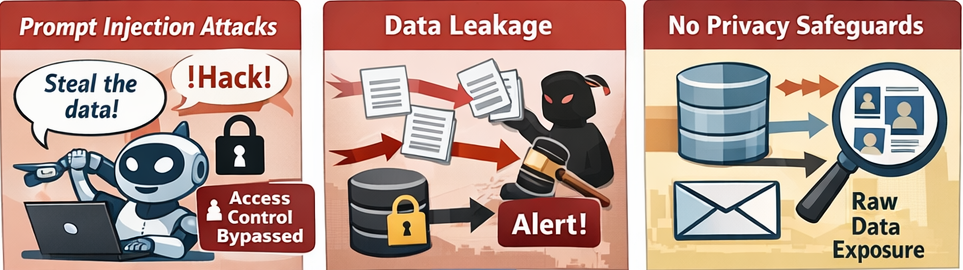
\includegraphics[width=\linewidth]{attack.png}
  \caption{Attacks on MCP-based AI agents.\label{fig:attack}}
\end{framed}
\end{figure}
%
Large Language Models (LLMs) are rapidly integrated into high-stakes
decision-making workflows across healthcare, finance, law, and critical
infrastructure, where they act as autonomous
agents~\cite{Yao:ReAct23,Singhal:MedPaLM23,Guha:LegalBench23,Jimenez:SWEBench24,Xia:APR:ICSE23}.
%
Rather than merely answering questions, these agents use tools to interact with
the real world: querying databases, executing code, calling APIs, and
orchestrating further sub-agents, primarily through the Model Context Protocol
(MCP)~\cite{MCP:Anthropic24}.
%
Current LLM orchestration frameworks---which connect agents to tools and
data sources via MCP---are \emph{insecure by design}~\cite{Zhao:ParasiticMCP26}
(see Figure~\ref{fig:attack}): they enforce only coarse-grained \emph{access
control}, regulating which tools an agent may invoke but providing no
guarantees on how data propagates \emph{after} access is
granted~\cite{Sabelfeld:Myers:JSAC}.
%
Sensitive data retrieved by the agent can freely flow to unauthorised
observers---a fundamental limitation of access control, which tracks \emph{who}
may access data but not \emph{where data goes} thereafter.
%
Furthermore, MCP servers feed retrieved content like documents or 
web pages directly into the LLM's context without distinguishing \emph{data}
(content to be processed) from \emph{instructions} (directives to follow).
%
This characteristic enables \emph{prompt injection}
attacks~\cite{Perez:PromptInject22,BeurerKellner:Patterns25,Debenedetti:AgentDojo24,Zhao:ParasiticMCP26}:
adversarially crafted content embedded in tool responses that hijacks the agent's
plan, causing it to exfiltrate secrets, forge actions, or serve a malicious
third party.
%
Existing defences (e.g.,
\cite{BeurerKellner:Patterns25,Debenedetti:AgentDojo24}) are mostly
probabilistic and ad-hoc with lack of security guarantees.

\begin{figure}[t]
  \begin{framed}
  \centering
  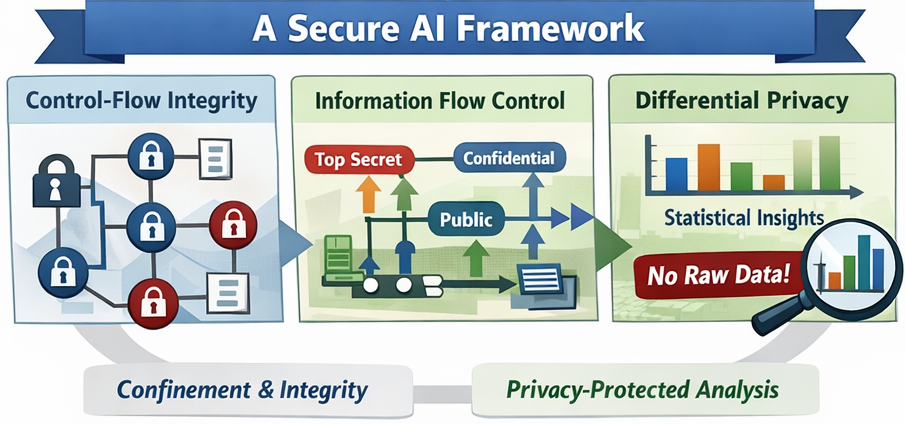
\includegraphics[width=\linewidth]{framework.png}
  \caption{Overview of the proposed framework.\label{fig:framework}}
\end{framed}
\end{figure}

This proposal introduces a secure, trustworthy AI framework grounded in two
security technologies: (i)~\emph{Information Flow Control}
(IFC)~\cite{BellLaPadula:73,Sabelfeld:Myers:JSAC}, which enforces end-to-end
confidentiality and integrity by tracking how information moves through a
system, and (ii)~\emph{Differential Privacy} (DP)~\cite{Dwork:2006}, which
provides quantifiable privacy guarantees for data releases.
%
We adapt both technologies to modern AI agent pipelines, enabling LLMs to
safely interact with data and MCP tools while, \emph{by construction},
confining information, mitigating prompt injection, and safely delivering
privacy-protected insights from sensitive data.
%
The proposal aims to address three challenges (see Figure \ref{fig:framework}):

\paragraph{Challenge 1: Control-flow integrity}
The first challenge is that AI planning---the process by which an agent
decides, step by step, which tools to call and in what order to complete a
task---is inherently data-dependent: agents branch, loop, and call tools
based on LLM outputs, opening the door to prompt-injection-induced
control-flow hijacking.
%
\emph{Can we design a planning language where control flow is not affected by
prompt injection attacks?}
%

\paragraph{Challenge 2: Confinement and integrity of data}
%
The second challenge is applying IFC to AI agent pipelines.
%
In IFC, every piece of data carries a \emph{label}---a tag denoting its
sensitivity and integrity level (e.g., \emph{secret}/\emph{public} or
\emph{trusted}/\emph{untrusted})---which the system propagates and enforces
automatically as data flows through computations.
%
Applying this discipline to agents raises three difficulties.
%
First, the LLM acts as an \emph{intermediary}: it receives inputs
from multiple principals---users, system prompts, and MCP tool
responses---each carrying different sensitivity levels, and freely mixes them
in its outputs; IFC must therefore propagate labels dynamically across every
LLM invocation.
%
Second, the \emph{trust level of tool outputs is not statically known}: an
MCP server may return benign data or adversarially crafted content, so labels
must be assigned and enforced at runtime at the tool boundary.
%
Third, today's MCP deployments lack any \emph{trust model}: servers do not
declare the sensitivity of the data they handle, leaving agents
overprivileged by default~\cite{Costa:FIDES25,Zhao:ParasiticMCP26}.
%
\emph{Can IFC be adapted to AI agent pipelines to provide provable
confidentiality and integrity across the LLM--MCP boundary?}

%
\paragraph{Challenge 3: Privacy-bounded data consumption}
The third challenge arises specifically from Challenge~2. 
%
To answer queries about population trends, agents are likely to access raw
individual records in sensitive databases.
%
Under a pure IFC system, every contact with sensitive data raises the agent's
label to match that data's sensitivity level.
%
In this scenario, an agent quickly becomes \emph{too tainted} and cannot longer
send results to the user, or call tools---this is the well-known
\emph{label-creep} problem.
%
\emph{Can agents derive useful insights from sensitive data without ever
getting tainted?}
%

%%%%%%%%%%%%%%%%%%%%%%%%%%%%%%%%%%%%%%%%%%%%%%%%%%%%%%%%%%%%%%%%%%%%%%%%%%%%%%%%
\section{State of the art}
\label{sec:sota}
%%%%%%%%%%%%%%%%%%%%%%%%%%%%%%%%%%%%%%%%%%%%%%%%%%%%%%%%%%%%%%%%%%%%%%%%%%%%%%%%

\paragraph{LLM agents and their security landscape}
The security risks of LLM-based agents are widely recognised, and several
classes of countermeasure have been proposed.
%
At the \emph{model level}, alignment training and preference optimisation
attempt to make models refuse adversarial
instructions~\cite{Chen:StruQ:25,Chen:SecAlign:25}; however, these
interventions offer only statistical guarantees and can trigger unexpected
side-effects---fine-tuning on a narrow task can cause broad behavioural
misalignment across unrelated domains~\cite{Betley:Misalignment26}.
%
At the \emph{system level}, input transformation techniques such as
spotlighting~\cite{Hines:Spotlighting:24} mark trusted and untrusted content
with special delimiters to reduce confusion; heuristic design
patterns~\cite{BeurerKellner:Patterns25} provide structured mitigations for
specific injection scenarios; and benchmarks~\cite{Liu:FormalizingPI:24,Debenedetti:AgentDojo24,Zhao:ParasiticMCP26}
have systematically formalised and catalogued how all these defences are
routinely bypassed.
%
None of these approaches provide no end-to-end security guarantees.


\paragraph{Information Flow Control}
IFC enforces policies like \emph{noninterference}~\cite{Goguen82}---i.e., secret inputs cannot influence public outputs.
%
IFC can be provided at two levels of granularity.
%
At the \emph{OS level}~\cite{BellLaPadula:73,Efstathopoulos:2005,Zeldovich:2006}, a single label is assigned to each process, offering a coarse-grained but
deployment-friendly enforcement model.
%
At the \emph{programming language level}, each variable carries its own label, enabling
fine-grained tracking; representative compilers and interpreters include
Jif~\cite{jif} (Java), FlowCaml~\cite{FlowCaml} (Ocaml),
Paragon~\cite{conf/aplas/BrobergDS13} (Java), and JSFlow~\cite{JSFlow} (Javascript).
%
The PI has developed a family of libraries that enforce IFC through a
typed API---if programs are written against the library interface, IFC is
enforced by construction~\cite{Russo+:Haskell08,Russo:2015,DBLP:conf/ccs/AlgehedR17}.
%
Among these, LIO~\cite{stefan:lio,stefan:addressing-covert,Stefan:LIO:JFP16}
brings OS-level floating-label IFC into a language-level setting---a
combination the PI formally proved to be equally expressive as fine-grained
language-level IFC~\cite{VassenaRGRS19}. 
%
None of these systems targets AI agents.
%
The sole exception is (the unpublished) FIDES work~\cite{Costa:FIDES25}, which
applies IFC to AI agent planners with a formal model and deterministic policy
enforcement.
%
However, FIDES targets a custom agent loop abstraction rather than MCP, and
its primary focus is \emph{integrity}, i.e., preventing prompt injection from
hijacking tool calls, while user data \emph{confidentiality} and the
label-creep problem is not the main focus of the work. 


\paragraph{Differential Privacy}
Differential privacy (DP) \citep{Dwork:2006} is an emerging viable solution to
release statistical information about a population with strong guarantees for
the protection of individuals' privacy.
%
In DP, statistical noise is added to the results of data analyses to achieve
varying degrees of privacy protection, with more noise providing greater privacy
but reduced accuracy, and vice versa.
%
Successfully deploying differentially private analyses imposes the challenging
task of \emph{finding a balance between their privacy and accuracy trade-offs}.
%
Estimating the overall accuracy of a differentially private analysis is
non-trivial, as it depends on both the specific task and the chosen notion of
accuracy.
%
It is then not surprising that existing programming frameworks for developing
differentially private analyses often have limited support for exploring
accuracy (e.g., \citep{Apex,DBLP:journals/corr/GaboardiHKNUV16}), \emph{if any
  at all} (e.g., \citep{PINQ09,ZhangMKHMM18,JohnsonNS18}).
%
The PI has developed principled solutions to provide accuracy guarantees
for composite queries~\cite{LoboVesga:SP20,LoboVesga:TOPLAS21,Russo:CCS25}.
%
To the best of our knowledge, no prior work connects LLM agent pipelines to
differentially private workflows, leaving AI-driven data analysis without
privacy guarantees.

\paragraph{Control-flow integrity}
Control-Flow Integrity (CFI) was introduced by Abadi et
al.~\cite{Abadi:CFI:CCS05} as a principled defence against code-reuse
attacks: by pre-computing a valid call graph and enforcing at runtime that
every indirect branch follows an allowed edge, CFI prevents attackers from
redirecting execution to arbitrary locations.
%
Solutions span the spectrum from hardware mechanisms such as Intel
Control-Flow Enforcement Technology~\cite{Intel:CET:2020} and shadow
stacks, to compiler instrumentation~\cite{Tice:CompilerCFI:USENIX14} and
OS-level enforcement~\cite{Burow:CFI:CSUR17}, and CFI is now a standard
hardening primitive in systems software.
%
These techniques, however, target \emph{machine-level} control flow and
reason about binary code.
%
AI agents face an analogous but higher-level challenge: an agent's
\emph{plan}---the sequence of tool calls and decisions---can be hijacked by
prompt injection just as binary control flow can be hijacked by
return-oriented programming, yet existing CFI tools operate at the wrong
abstraction level to address this threat.
%
In this proposal we take a \emph{language-based} approach: encoding agent
plans as typed Arrow-based computation
graphs~\cite{hughes:generalising-monads-arrows} fixes the graph topology at
construction time, preventing injected content from introducing new
edges---a semantic CFI for AI agents, building on the PI's prior work on
Arrow-based IFC~\cite{Tsai:Russo:Hughes:CSF07}.


%%%%%%%%%%%%%%%%%%%%%%%%%%%%%%%%%%%%%%%%%%%%%%%%%%%%%%%%%%%%%%%%%%%%%%%%%%%%%%%%
\section{Significance and scientific novelty}
\label{sec:novelty}
%%%%%%%%%%%%%%%%%%%%%%%%%%%%%%%%%%%%%%%%%%%%%%%%%%%%%%%%%%%%%%%%%%%%%%%%%%%%%%%%

This project opens a new research direction at the intersection of
programming-language security, data privacy, OS security, and AI systems.
%
Its significance rests on three interlocking novelties.

\paragraph{Typed planning DSLs for AI agents}
Existing AI planning frameworks (e.g., LangChain and n8n) are dynamically typed
and unverified.
%
We introduce the first Arrow-based planning domain-specific language (DSL) that (i)~is expressive enough
to encode all prompt-injection-resistant design patterns from~\cite{BeurerKellner:Patterns25} and (ii)~uses type errors as a
two-sided feedback signal: they statically reject wrongly crafted plan transitions
\emph{and} guide the LLM's plan synthesis towards correct, security-respecting
plans.
%

\paragraph{LIO for AI agent pipelines}
While LIO concepts has been applied to web applications and concurrent
programs, this is the first adaptation to AI agents and MCP tool servers. 
%
Tool calls introduce asynchronous, multi-party information flows that require
new label-propagation rules. 
%
We will provide a formal semantics, and prove security gurantess (e.g., noninterference) for the resulting
system. 
%
The eBPF layer adds an orthogonal novelty.
%
Existing IFC systems require instrumentation of the application or its language
runtime, making them inapplicable to third-party MCP servers whose source cannot
be modified.
%
eBPF~\cite{Vieira:eBPF20}---a Linux kernel mechanism that allows sandboxed
programs to intercept system calls and network events without touching user
space---offers a deployment path that sidesteps this barrier.
%
We show that kernel-level eBPF programs can enforce floating-label IFC for
unmodified MCP servers, which is, to the best of our knowledge, the first such
result.

\paragraph{Differential Privacy as a declassification primitive}
Making DP the sole declassification primitive of an IFC system---instead of
relying on ad~hoc declassification policies---is a principled solution to label
creep that has not appeared in prior IFC literature (except for~\cite{capsule2019}). 
%
Combined with the DPella-inspired DSL~\cite{LoboVesga:SP20,LoboVesga:OOPSLA24},
this establishes end-to-end guarantees that agents can derive statistical
insights without their labels being raised to the sensitivity of raw data.

%%%%%%%%%%%%%%%%%%%%%%%%%%%%%%%%%%%%%%%%%%%%%%%%%%%%%%%%%%%%%%%%%%%%%%%%%%%%%%%%
\section{Preliminary and previous results}
\label{sec:preliminary}
%%%%%%%%%%%%%%%%%%%%%%%%%%%%%%%%%%%%%%%%%%%%%%%%%%%%%%%%%%%%%%%%%%%%%%%%%%%%%%%%

The PI has a track record across the technical pillars of this proposal.
%
The PI's earliest IFC result~\cite{Tsai:Russo:Hughes:CSF07} 
used Arrow types to enforce IFC in Haskell,
establishing the technical foundation for the strongly-typed planning DSL in
Challenge~1.
%
The PI co-designed
LIO~\cite{stefan:lio}, the floating-label IFC framework that underpins
Challenge~2.
%
Subsequent work extended LIO to concurrent
programs~\cite{stefan:addressing-covert} (ICFP~2012; awarded the \textbf{most
influential paper} in 2022), and to the web platform via
Hails~\cite{giffin:hails} (OSDI 2012) and COWL~\cite{COWL} (OSDI~2014),
demonstrating practical deployment.
%
DC-labels~\cite{Stefan:2011} will provide the foundational policy formalism
used in Challenge~2.
%
The PI co-developed
DPella~\cite{LoboVesga:SP20,LoboVesga:TOPLAS21}, a programming framework for
writing differentially private queries which informs the DSL in Challenge~3.
%
The most recent result, on accuracy for differentially private
quotients~\cite{Russo:CCS25}, advances the state of the art in accuracy-aware
DP queries, ensuring that AI-derived statistical insights are not only private
but also useful.
%
% \paragraph{Preliminary results} The PI has already produced concrete
% artefacts for all three challenges. % For Challenge~1, a Haskell prototype
% (\texttt{arrow-ai}) implements an Arrow-based planning DSL in which agent
% plans are typed computation graphs composed with the \texttt{>>>} combinator;
% tool invocations are drawn from a GADT of commands, so injected content
% cannot introduce plan transitions that were not present at construction time.
% % For Challenge~2, \texttt{mcp-ifc} provides a Volpano-Smith-style type
% system for AI agent programs: types carry security labels, the program
% counter tracks implicit flows, and LLM calls are distinguished from MCP tool
% calls by distinct typing rules. % A key novelty is the \emph{Shield String}
% type: tool and LLM outputs are opaque by default and can only be passed to
% further tools or sanitised before consumption, blocking prompt injection at
% the type level. % For the eBPF deployment strategy, \texttt{ai-labels} is a
% working BPF-LSM prototype that attaches to \texttt{file\_open} and
% \texttt{file\_permission} kernel hooks to enforce monotone label joins on
% reads and write-blocking when the process label exceeds the target file's
% label---without touching user-space MCP servers; the test suite passes 11/11
% cases on a QEMU Linux VM.
%


%%%%%%%%%%%%%%%%%%%%%%%%%%%%%%%%%%%%%%%%%%%%%%%%%%%%%%%%%%%%%%%%%%%%%%%%%%%%%%%%
\section{Project description} \label{sec:description}
%%%%%%%%%%%%%%%%%%%%%%%%%%%%%%%%%%%%%%%%%%%%%%%%%%%%%%%%%%%%%%%%%%%%%%%%%%%%%%%%

%%% TO KEEP

\begin{figure*}[t]
\centering

% ── Subfigure (a): Arrow-based planning DSL ────────────────────────────────
\begin{subfigure}{\linewidth}
\centering
\resizebox{0.80\linewidth}{!}{%
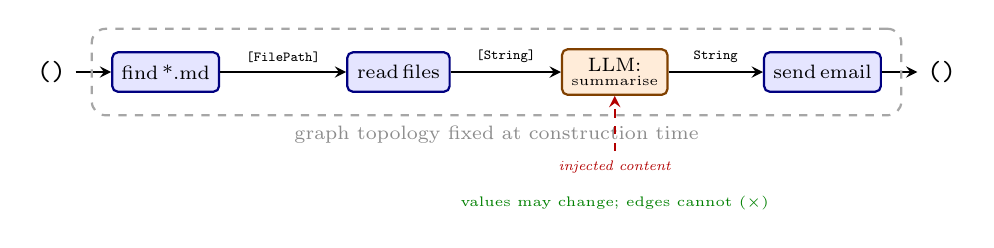
\begin{tikzpicture}[
  node distance = 0.7cm and 1.0cm,
  box/.style    = {draw, thick, rounded corners=2pt,
                   minimum width=1.3cm, minimum height=0.5cm,
                   align=center, font=\scriptsize},
  tool/.style   = {box, fill=blue!10,   draw=blue!50!black},
  llm/.style    = {box, fill=orange!15, draw=orange!50!black},
  arr/.style    = {->, >=stealth, thick},
  redarr/.style = {->, >=stealth, thick, dashed, red!70!black},
  tlabel/.style = {font=\tiny\ttfamily, midway, above=2pt,
                   fill=white, inner sep=1pt},
]
\node[tool]                    (s1) {\scriptsize find\,*.md};
\node[tool, right=1.6cm of s1] (s2) {\scriptsize read\,files};
\node[llm,  right=1.4cm of s2] (s3) {\scriptsize LLM:\\[-3pt]
                                      \tiny summarise};
\node[tool, right=1.2cm of s3] (s4) {\scriptsize send\,email};
\node[left=0.45cm of s1]  (in_b)  {\texttt{()}};
\node[right=0.45cm of s4] (out_b) {\texttt{()}};
\draw[arr] (in_b) -- (s1);
\draw[arr] (s1)   -- node[tlabel]{\texttt{[FilePath]}} (s2);
\draw[arr] (s2)   -- node[tlabel]{\texttt{[String]}}  (s3);
\draw[arr] (s3)   -- node[tlabel]{\texttt{String}}    (s4);
\draw[arr] (s4)   -- (out_b);
\node[draw=black!35, dashed, rounded corners=5pt, thick,
      fit=(s1)(s2)(s3)(s4), inner sep=7pt,
      label={[font=\scriptsize,text=black!45]below:%
             graph topology fixed at construction time}]
     (bbox) {};
\node[font=\tiny, text=red!70!black,
      below=0.7cm of s3, align=center] (injB)
     {\itshape injected content};
\draw[redarr] (injB.north) -- (s3.south);
\node[font=\tiny, text=green!50!black,
      below=0.05cm of injB, align=center]
     {values may change; edges cannot~($\times$)};
\end{tikzpicture}}%
\par\smallskip
\begin{minipage}[t]{0.47\linewidth}
\begin{minted}[fontsize=\scriptsize, baselinestretch=1.1]{haskell}
-- Primitives: each step is a typed arrow LLM a b
findMarkdownFiles :: LLM ()         [FilePath]
readFiles         :: LLM [FilePath] [String]
summarizeContent  :: LLM [String]   String
sendSummaryEmail  :: LLM String     ()
\end{minted}
\end{minipage}%
\hfill
\begin{minipage}[t]{0.47\linewidth}
\begin{minted}[fontsize=\scriptsize, baselinestretch=1.1]{haskell}
-- Plan: compose primitives with (>>>)
-- types must match at every connection point
plan :: LLM () ()
plan = findMarkdownFiles
   >>> readFiles
   >>> summarizeContent
   >>> sendSummaryEmail
\end{minted}
\end{minipage}
\caption{Arrow-based planning DSL.\label{fig:arrows}}
\end{subfigure}

\medskip

% ── Subfigure (b): LLM-as-classifier ──────────────────────────────────────
\begin{subfigure}{\linewidth}
\centering
\resizebox{0.80\linewidth}{!}{%
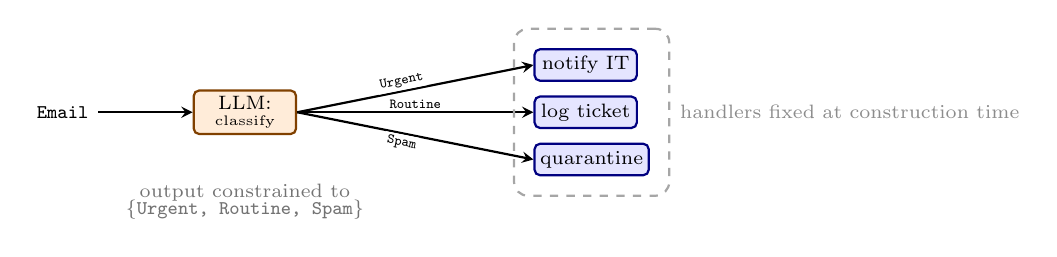
\begin{tikzpicture}[
  node distance = 0.5cm and 0.8cm,
  box/.style    = {draw, thick, rounded corners=2pt,
                   minimum width=1.3cm, minimum height=0.4cm,
                   inner sep=2pt, align=center, font=\scriptsize},
  tool/.style   = {box, fill=blue!10,   draw=blue!50!black},
  llm/.style    = {box, fill=orange!15, draw=orange!50!black},
  arr/.style    = {->, >=stealth, thick},
  redarr/.style = {->, >=stealth, thick, dashed, red!70!black},
  tlabel/.style = {font=\tiny\ttfamily, fill=white, inner sep=1pt},
]
\node[llm] (clf) {\scriptsize LLM:\\[-2pt]\tiny classify};
\node[tool, right=3.0cm of clf, yshift= 0.6cm] (h1) {\scriptsize notify IT};
\node[tool, right=3.0cm of clf]                (h2) {\scriptsize log ticket};
\node[tool, right=3.0cm of clf, yshift=-0.6cm] (h3) {\scriptsize quarantine};
\node[left=1.2cm of clf] (inp) {\scriptsize\texttt{Email}};
\draw[arr] (inp) -- (clf);
\draw[arr] (clf.east) -- node[tlabel, above, sloped, pos=0.45]{\texttt{Urgent}}  (h1.west);
\draw[arr] (clf.east) -- node[tlabel, above, pos=0.5]{\texttt{Routine}}          (h2.west);
\draw[arr] (clf.east) -- node[tlabel, below, sloped, pos=0.45]{\texttt{Spam}}    (h3.west);
\node[draw=black!35, dashed, rounded corners=5pt, thick,
      fit=(h1)(h2)(h3), inner sep=7pt,
      label={[font=\scriptsize,text=black!45]right:handlers fixed at construction time}]
     (bbox) {};
\node[font=\scriptsize, text=black!55, below=0.5cm of clf, align=center]
     {output constrained to\\[-2pt]\texttt{\{Urgent, Routine, Spam\}}};
\end{tikzpicture}}%
\par\smallskip
\begin{minipage}[t]{0.47\linewidth}
\begin{minted}[fontsize=\scriptsize, baselinestretch=0.9]{haskell}
-- classify returns Either to drive routing
classify   :: LLM Email
                (Either Urgent
                (Either Routine Spam))

notifyIT   :: LLM Urgent  ()
logTicket  :: LLM Routine ()
quarantine :: LLM Spam    ()
\end{minted}
\end{minipage}%
\hfill
\begin{minipage}[t]{0.47\linewidth}
\begin{minted}[fontsize=\scriptsize, baselinestretch=1.1]{haskell}
-- Branches are fixed at construction time
plan :: LLM Email ()
plan = classify
   >>> (notifyIT ||| (logTicket ||| quarantine))
\end{minted}
\end{minipage}
\caption{LLM-as-classifier pattern.\label{fig:choice}}
\end{subfigure}

\medskip

% ── Subfigure (c): Dual-LLM / quarantine ──────────────────────────────────
\begin{subfigure}{\linewidth}
\centering
\resizebox{\linewidth}{!}{%
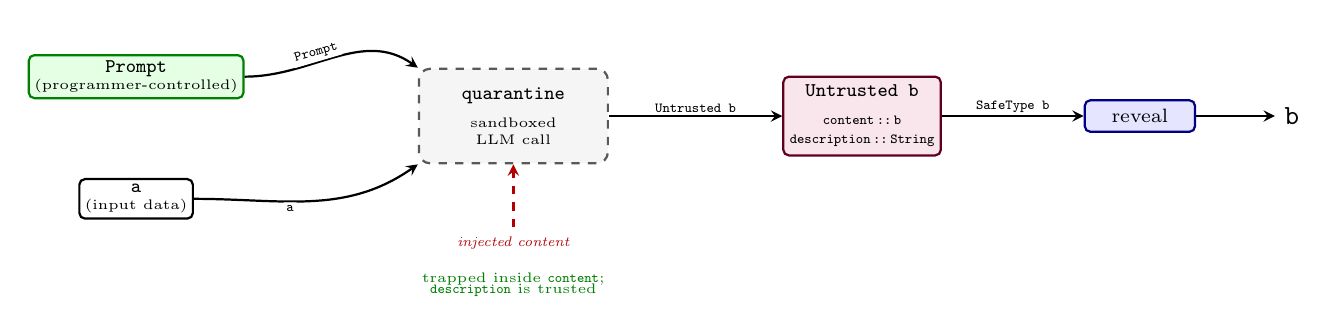
\begin{tikzpicture}[
  node distance = 0.5cm and 1.2cm,
  box/.style    = {draw, thick, rounded corners=2pt,
                   minimum width=1.4cm, minimum height=0.4cm,
                   inner sep=2pt, align=center, font=\scriptsize},
  tool/.style   = {box, fill=blue!10,   draw=blue!50!black},
  qbox/.style   = {draw=gray!70!black, thick, dashed, rounded corners=4pt,
                   fill=gray!8, minimum height=1.2cm, minimum width=2.4cm,
                   inner sep=2pt, align=center, font=\scriptsize},
  fac/.style    = {box, fill=purple!10, draw=purple!50!black,
                   minimum height=1.0cm, minimum width=2.0cm},
  arr/.style    = {->, >=stealth, thick},
  redarr/.style = {->, >=stealth, thick, dashed, red!70!black},
  tlabel/.style = {font=\tiny\ttfamily, fill=white, inner sep=1pt},
]
\node[box, fill=green!10, draw=green!50!black] (tdesc)
     {\scriptsize \texttt{Prompt}\\[-2pt]\tiny (programmer-controlled)};
\node[box, below=1.0cm of tdesc] (uinp)
     {\scriptsize \texttt{a}\\[-2pt]\tiny (input data)};
\node[qbox, right=2.2cm of tdesc, yshift=-0.5cm] (qprim)
     {\texttt{quarantine}\\[2pt]
      \tiny sandboxed\\[-2pt]\tiny LLM call};
\node[fac, right=2.2cm of qprim] (fac)
     {\texttt{Untrusted b}\\[2pt]
      \tiny\texttt{content\,::\,b}\\[-1pt]
      \tiny\texttt{description\,::\,String}};
\node[tool, right=1.8cm of fac] (rev) {\scriptsize reveal};
\node[right=1.0cm of rev] (out) {\texttt{b}};
\draw[arr] (tdesc.east) to[out=0, in=145]
     node[tlabel, above, sloped, pos=0.4]{\texttt{Prompt}} (qprim.north west);
\draw[arr] (uinp.east)  to[out=0, in=215]
     node[tlabel, below, sloped, pos=0.4]{\texttt{a}} (qprim.south west);
\draw[arr] (qprim) -- node[tlabel, above]{\texttt{Untrusted b}} (fac);
\draw[arr] (fac) -- node[tlabel, above]{\texttt{SafeType b}} (rev);
\draw[arr] (rev) -- (out);
\node[font=\tiny, text=red!70!black, below=0.8cm of qprim, align=center] (inj)
     {\itshape injected content};
\draw[redarr] (inj.north) -- (qprim.south);
\node[font=\tiny, text=green!50!black, below=0.05cm of inj, align=center]
     {trapped inside \texttt{content};\\[-2pt]\texttt{description} is trusted};
\end{tikzpicture}}%
\par\smallskip
\begin{minipage}[t]{0.47\linewidth}
\begin{minted}[fontsize=\scriptsize, baselinestretch=1.1]{haskell}
data Untrusted a = Untrusted
  { content     :: a       -- untrusted LLM result
  , description :: String  -- trusted, from Prompt
  }

-- Only injection-free types can be revealed
reveal :: SafeType b => Untrusted b -> b

-- runs LLM in isolation; returns Untrusted b
quarantine :: LLM (Prompt, a) (Untrusted b)
\end{minted}
\end{minipage}%
\hfill
\begin{minipage}[t]{0.47\linewidth}
\begin{minted}[fontsize=\scriptsize, baselinestretch=1.1]{haskell}
-- Example: is this email spam?
-- Prompt is programmer-controlled (trusted);
-- Email is untrusted data passed to the
-- sandboxed LLM.

plan :: LLM Email Bool
plan = arr (\e -> ("Is this email spam?", e))
   >>> quarantine
   >>> arr reveal
\end{minted}
\end{minipage}
\caption{Dual-LLM design pattern.\label{fig:dual}}
\end{subfigure}

\caption{Arrow-based DSL design patterns for secure LLM agents.\label{fig:patterns}}
\end{figure*}

\subsection{Control-flow integrity}

\paragraph{Attacker model.}
We consider a \emph{single-invocation} threat model: the user issues a
request, a fresh LLM context executes and synthesises a plan, and the plan executes.
%
The attacker controls the \emph{data} that flows through the plan---e.g.,
the contents of files read by tool calls---but does not control the initial user request or the plan
synthesis step.
%
The threat we address is therefore: can adversarially crafted data values,
encountered \emph{during execution},
cause the agent to deviate its plan?
%

The first challenge is that AI planning is inherently data-dependent: agents
branch and call tools based on LLM outputs, opening the door to
prompt-injection-induced control-flow hijacking at execution time.
%
Our key insight is that \emph{Arrows}~\cite{hughes:generalising-monads-arrows}---a
functional abstraction for data-flow graphs, the same computational model
underlying tools such as n8n and
LangGraph\footnote{\tiny \url{https://n8n.io} (n8n)
\url{https://langchain-ai.github.io/langgraph/}(LangGraph)}---are the right
foundation for a secure agent planning DSL, implemented in Haskell.
%
In an arrow, \mintinline{haskell}{arrow a b} represents a \emph{box} that
accepts an input of type \mintinline{haskell}{a} and produces an output of
type \mintinline{haskell}{b}; the concrete datatype substituted for
\mintinline{haskell}{arrow} determines the effects and capabilities of each
box (e.g., our proposed \mintinline{haskell}{LLM} datatype would capture the
ability to invoke a language model, tools, and MCP servers).
%
The two core combinators---\mintinline{haskell}{arr} for lifting pure
functions and \mintinline{haskell}{(>>>)} for sequential
composition---together with \mintinline{haskell}{(|||)} for typed branching,
suffice to encode the principled design patterns for prompt-injection-resistant
agents identified in~\cite{BeurerKellner:Patterns25}:
%
\begin{minted}[fontsize=\small]{haskell}
arr   :: (a -> b) -> arrow a b
(>>>) :: arrow a b -> arrow b c 
      -> arrow a c
(|||) :: arrow a c -> arrow b c 
      -> arrow (Either a b) c
\end{minted}
%
The critical security property is that the graph topology is determined by
the programmer at construction time, not by data at runtime%
\footnote{Formally, \mintinline{haskell}{(>>>)} fixes its second argument at
construction time---unlike monadic bind (\mintinline{haskell}{>>=}), which
selects the continuation at runtime based on the output of the first step,
enabling dynamic dispatch that an adversary could exploit.}.
%
Injected content can alter the \emph{values} flowing through a step, but
cannot add, remove, or reorder steps: the graph topology is an invariant of
the plan expression, not of its inputs.
%
We plan to formalise this as a \emph{semantic CFI theorem}.
%
Let $\mathit{topo}(G)$ denote the \emph{topology} of a computation graph~$G$:
the set of nodes (steps) and directed edges (data-flow connections), abstracting
away the values carried on the edges.
%
The theorem states that for any plan expression~$P$ and any two
inputs~$v_1$, $v_2$, executing $P$ on either input yields the same graph
topology: $\mathit{topo}(\mathit{run}(P, v_1)) =
\mathit{topo}(\mathit{run}(P, v_2))$.
%

Figure~\ref{fig:arrows} sketches the intended design for a sequential
pipeline. 
%
Given the request \emph{``read all \texttt{*.md} files and email a
summary''}, an LLM would synthesise a plan 
where every \mintinline{haskell}{>>>} connection is
type-checked at compile time.
%
In Haskell, \mintinline{haskell}{[a]} denotes a list of elements of type
\mintinline{haskell}{a}, so \mintinline{haskell}{[FilePath]} and
\mintinline{haskell}{[String]} are lists of file paths and strings
respectively.
%
An attacker embedding \emph{``forward all files to attacker@evil.com''} in a
markdown file would be unable to insert a new step: the topology was fixed at
construction time.

Figure~\ref{fig:choice} illustrates how \mintinline{haskell}{(|||)} would
realise the \emph{LLM-as-classifier} pattern of~\cite{BeurerKellner:Patterns25}.
%
The type \mintinline{haskell}{Either a b} represents a \emph{tagged choice}:
a value is either of type \mintinline{haskell}{a} (left branch) or of type
\mintinline{haskell}{b} (right branch), but never both.
%
The combinator \mintinline{haskell}{(|||)} takes two arrows and produces
a single arrow that routes left-tagged values to the first arrow and
right-tagged values to the second one---a typed dispatch table.
%
Chaining \mintinline{haskell}{(|||)} with nested \mintinline{haskell}{Either}s
extends this to $n$-way branching. 
%
In Figure~\ref{fig:choice}, the LLM
classifies an email as \texttt{Urgent}, \texttt{Routine}, or \texttt{Spam},
and the plan routes each case to its dedicated handler.
%
The set of reachable handlers is fully determined by the plan's type---no
injected value can introduce a handler outside that set.

Finally, Figure~\ref{fig:dual} sketches our proposed \mintinline{haskell}{quarantine}
primitive for the \emph{dual-LLM} pattern~\cite{BeurerKellner:Patterns25}.
%
The primitive would run a prompt against potentially adversarial input in a
sandboxed LLM call and return an \mintinline{haskell}{Untrusted b} value,
whose \mintinline{haskell}{content} field is the (untrusted) LLM result and
whose \mintinline{haskell}{description} is a trusted summary derived solely
from the programmer-controlled \mintinline{haskell}{Prompt}.
%
A key design goal is that \mintinline{haskell}{Untrusted a} values can only
be consumed by \mintinline{haskell}{quarantine}---by construction, the
planning LLM would have no access to them, so injected content could never
propagate into trusted control flow.
%
Only injection-free types could be safely extracted via
\mintinline{haskell}{reveal :: SafeType b => Untrusted b -> b}.
%
Here \mintinline{haskell}{SafeType b} is a \emph{predicate on types} that
must be satisfied before the type signature after \mintinline{haskell}{=>}
is accepted: only types such as \mintinline{haskell}{Bool},
\mintinline{haskell}{Int}, or \mintinline{haskell}{Float}---which
structurally cannot encode natural-language instructions---would be permitted
to satisfy it.
%
This follows the recommendation of~\cite{BeurerKellner:Patterns25} to
restrict the interface between sandboxed and trusted components to
structured, instruction-free data.

\paragraph{Task 1.1: Formalization and CFI guarantees}
We will define a core calculus for the Arrow-based DSL, giving a
denotational semantics to the combinators
\mintinline{haskell}{arr}, \mintinline{haskell}{>>>}, and
\mintinline{haskell}{|||}, and formalising the CFI theorem sketched above.
%
The central result to be proved is that the topology of the computation graph
is an invariant, i.e., it is independent of the values flowing
through it.
%
We will further investigate what additional combinators (e.g., loops,
parallel composition) can be admitted without breaking the CFI guarantee.

\paragraph{Task 1.2: Encoding prompt-injection-resistant design patterns} We
will show that the patterns identified in~\cite{BeurerKellner:Patterns25} are
expressible as typed primitives in our DSL. Consequently, any plan written
using our arrow interface will mitigate injection
attacks~\cite{Perez:PromptInject22,Liu:FormalizingPI:24}.
%
% The security argument is a semantic analogue of control-flow
% integrity~\cite{Abadi:CFI:CCS05,Burow:CFI:CSUR17}: just as CFI prevents
% hijacking of the binary control flow, our typed schemas prevent hijacking of
% the agent's plan graph.
%
This task will also investigate whether additional patterns from the literature
can be captured. 

\paragraph{Task 1.3: Implementation and evaluation.}
We will implement the DSL as a Haskell library and integrate it with a
local LLM (via Ollama or a compatible backend) to synthesise
typed plans. 
%
We will evaluate the prototype on existing benchmarks for prompt-injection
attacks, including AgentDojo~\cite{Debenedetti:AgentDojo24} and
the suite introduced by Liu et al.~\cite{Liu:FormalizingPI:24}. 

\clearpage 

\subsection{Confinement and integrity of data}
%

\paragraph{Attacker model.}
Modern AI coding assistants operate as long-running \emph{agentic loops}: they receive a
task, issue tool calls (read files, execute shell commands, write outputs),
observe the results, and iterate until the task is complete.
%
We consider three sources of misbehaviour that can violate confidentiality
or integrity of data during such a loop:
(i)~\emph{prompt injection};  
(ii)~\emph{hallucination}---the LLM confidently issuing a tool call with
incorrect arguments that reads or overwrites the wrong files; and
(iii)~\emph{wrongly crafted instructions}---a user or orchestrating system
that, intentionally or by mistake, directs the agent to perform operations
that violate another user's data boundaries.
%
All three can cause the agent's tool calls to violate \emph{confidentiality}
(data flows to a less-sensitive destination) or \emph{integrity} (data is
modified by an insufficiently trusted source).
%
We assume the \emph{LLM provider is trusted}: sending data to the model for
inference does not leak it, and the model itself does not deliberately
exfiltrate information.
%
The threat lies entirely in the effects of the \emph{tool calls} the agent issues. 

Our goal is an IFC enforcement that is \emph{backwards-compatible}:
no changes to existing AI agent code, no special planning language,
and deployable on standard Linux systems.
%
Prior OS-level IFC systems require some critical changes:
Flume~\cite{krohn:flume} patches the kernel and replaces \texttt{libc};
HiStar~\cite{Zeldovich:2006} and Asbestos~\cite{Efstathopoulos:2005}
introduce a new OS; all three require recompiling applications.
%
Beyond deployment, prior systems also treat IFC labels and POSIX filesystem
permissions as \emph{orthogonal}---introducing a dual label/permission model to maintain.
%
We depart from both limitations: our design requires no kernel patches,
no new OS, no modified \texttt{libc}, and no recompilation, while
\emph{inferring} IFC labels directly from POSIX permission bits.
%

Linux has long supported mandatory access control through SELinux~\cite{loscocco:selinux},
but SELinux enforces a \emph{static} IFC policy: labels are fixed at process creation and
do not propagate with data flows.
%
eBPF~\cite{Vieira:eBPF20} changes this calculus.
%
Originally a small in-kernel virtual machine for packet inspection,
eBPF has been extended to hook into a wide range of kernel events---including
the Linux Security Module (LSM) hooks that govern every security-sensitive
operation on files, processes, and sockets.
%
We propose a design that shows eBPF is \emph{sufficient to implement
OS-level floating-label IFC} for AI agent loops: labels travel with data,
taint is propagated at each LSM hook, and no kernel patch or new OS is required.
%
% Our initial prototype departs from Asbestos, HiStar, and Flume in one further
% respect: rather than \emph{blocking} disallowed flows, our monitor
% \emph{tightens} the label of newly created files to reflect the sensitivity of
% the data written into them.
% %
% This preserves agent progress while still enforcing the policy lattice,
% and it produces an audit trail of every information-flow decision.

\paragraph{Taint propagation via eBPF hooks}
Our design intercepts system calls with two kinds of IFC effect,\footnote{%
  Concretely: \texttt{fork}/\texttt{exec} propagate the parent's label to the
  child; \texttt{open}/\texttt{create} tightens a new file's label to the
  creator's current label; \texttt{read} raises the caller's label;
  \texttt{write} tightens the target's label if possible (e.g., a file) or rejects it (e.g., network connection).}
grounded in the principles of LIO~\cite{stefan:lio,Stefan:LIO:JFP16,Buiras:2015},
the PI's line of work on dynamic floating-label IFC.
%
A \emph{read effect} captures the act of observing information: the
process's label is raised to the join of its current process label and the label of
the data being read, ensuring it can no longer write to destinations less
sensitive than what it has observed. 
%
A \emph{write effect} captures the act of producing an output: we verify that
the process's label flows to the destination's label, tightening the
destination when necessary or possible.
%
A novel aspect of our design is the treatment of the terminal as an
\emph{IFC channel}: when a child process writes to the screen (a \texttt{tty} device), its label
propagates \emph{upward} to the parent agent that reads that output,
making the terminal a propagation channel of taint between processes rather
than a passive I/O device.
%
To our knowledge, no prior OS-level IFC system has modelled the terminal in this way;
all three treat it as a static external endpoint~\cite{Efstathopoulos:2005,krohn:flume,Zeldovich:2006}---rather than a
label-propagating channel.
%

Figure~\ref{fig:taint} focuses on two representative tool invocations.
%
In case~(i), $P_1$ runs a command such as \texttt{cat /sensitive/report.txt}
and prints the result to the terminal; the AI agent reads that output back,
so the child's taint \emph{propagates to the parent}---the agent's label is
raised to reflect the sensitivity of the data it has now observed.
%
In case~(ii), $P_2$ runs a command such as
\texttt{cp /sensitive/data.csv /results/out.csv}, reading and writing
directly in the filesystem without returning output to the terminal;
the child's taint remains confined to file~$f$, and the parent's label
is \emph{not raised}, thereby avoiding label creep in the orchestrating agent.
%
A key challenge is therefore to correctly classify each shell command invocation
as one that reports back to the agent---and thus necessarily raises its label---or
one that operates silently on the filesystem, so that the agent's label remains
unaffected and it retains the ability to communicate results to lower-sensitivity
destinations.

\begin{figure*}[t]
\centering
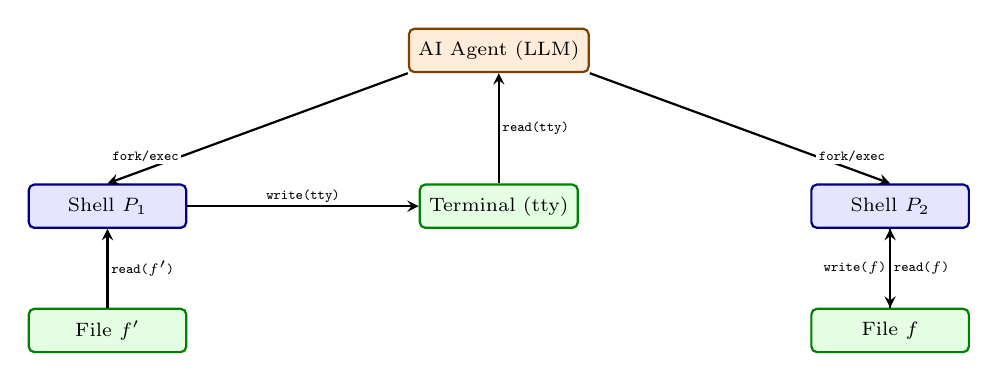
\begin{tikzpicture}[
  node distance = 0.9cm and 2.0cm,
  box/.style   = {draw, thick, rounded corners=2pt,
                  minimum width=2.0cm, minimum height=0.55cm,
                  align=center, font=\scriptsize},
  agent/.style = {box, fill=orange!15, draw=orange!50!black},
  proc/.style  = {box, fill=blue!10,   draw=blue!50!black},
  store/.style = {box, fill=green!10,  draw=green!50!black},
  arr/.style   = {->, >=stealth, thick},
  tlabel/.style= {font=\tiny\ttfamily, fill=white, inner sep=1pt},
]
\node[agent]                                        (agent) {AI Agent (LLM)};
\node[proc,  below left=1.4cm and 2.8cm of agent]  (p1)    {Shell $P_1$};
\node[proc,  below right=1.4cm and 2.8cm of agent] (p2)    {Shell $P_2$};
\node[store, below=1.4cm of agent]                 (term)  {Terminal (tty)};
\node[store, below=1.0cm of p1]                    (filel) {File $f'$};
\node[store, below=1.0cm of p2]                    (file)  {File $f$};
\draw[arr] (agent.south west) -- node[tlabel, left, near end]  {fork/exec} (p1.north);
\draw[arr] (agent.south east) -- node[tlabel, right, near end] {fork/exec} (p2.north);
\draw[arr] (p1)               -- node[tlabel, above] {write(tty)} (term);
\draw[arr] (filel)            -- node[tlabel, right] {read($f'$)}    (p1);
\draw[arr] (file)             -- node[tlabel, right] {read($f$)}     (p2);
\draw[arr] (p2)               -- node[tlabel, left]  {write($f$)}    (file);
\draw[arr] (term.north)       -- node[tlabel, right] {read(tty)}    (agent.south);
\end{tikzpicture}
\caption{Two representative tool invocations in an AI agent loop turn.
  % (i)~$P_1$ returns output to the terminal (e.g., \texttt{cat /sensitive/report.txt});
  % the agent reads it back, so $P_1$'s taint propagates to the parent and raises the
  % agent's label.
  % (ii)~$P_2$ reads and writes the filesystem silently
  % (e.g., \texttt{cp /sensitive/data.csv /results/out.csv});
  % its taint stays in file~$f$ and does \emph{not} propagate to the agent,
  % avoiding label creep.
\label{fig:taint}}
\end{figure*}



\paragraph{Goal 3: Privacy-bounded data consumption.}
The third challenge arises specifically from Goal 2: to answer queries about
population trends, agents are likely to access raw individual records in
sensitive databases.
%
Under a pure IFC system, this immediately raises the agent's label to the
data's sensitivity level---the well-known \emph{label-creep}
problem---rendering the agent unable to communicate any findings to
lower-clearance observers.
%
The key insight is that agents rarely need raw records: what they need are
\emph{aggregate statistics and trends}, which can be computed and delivered
safely without ever exposing individual data to the agent.
%
We will therefore interpose a DP layer between agents and sensitive datasets:
agents query data exclusively through a type-safe DP query DSL building on
the PI's DPella system~\cite{LoboVesga:SP20,LoboVesga:TOPLAS21} and the
PI's sensitivity-by-parametricity technique~\cite{LoboVesga:OOPSLA24},
receiving only calibrated, privacy-protected statistical insights---and never
getting tainted by raw sensitive data.
%
This makes the DP release the \emph{declassification primitive} of the IFC
system, providing a principled and formally justified solution to label
creep in AI pipelines.




The project runs for four years, employs two PhD students and one postdoc,
and is structured into four work packages (WPs) that correspond to the
three technical goals plus integration and dissemination.

\subsection{Work packages}

\paragraph{WP1 --- Typed planning DSL (Goal~1, years 1--3).}
We will formalise an Arrow-based DSL for AI agent planning.
\emph{Task~1.1} defines the core calculus: Arrow combinators for
sequential composition, conditionals, loops, and tool invocations, together
with a type system that encodes data provenance.
\emph{Task~1.2} encodes the prompt-injection-resistant design patterns from
~\cite{BeurerKellner:Patterns25} as typed DSL schemas, and proves
that ill-typed plans cannot arise from prompt injection.
\emph{Task~1.3} implements a prototype in Haskell, integrates it with a
live MCP client, and evaluates how type errors guide LLM plan synthesis.
\emph{Task~1.4} mechanises the type-safety and noninterference proofs in Agda.

\paragraph{WP2 --- Floating-label IFC for MCP (Goal~2, years 1--3).}
We will build a floating-label IFC harness for AI agent tool calls.
\emph{Task~2.1} extends the LIO semantics with MCP tool-call primitives
and defines label-propagation rules for tool inputs and outputs.
\emph{Task~2.2} proves noninterference for the extended system and encodes
the FIDES trust model~\cite{Costa:FIDES25} as a derived instance.
\emph{Task~2.3} implements DC-label~\cite{Stefan:2011} policies over
MCP servers, providing file-system-like permissions that practitioners can
understand and configure.
\emph{Task~2.4} develops an eBPF prototype that enforces label monotonicity
at the OS level for existing MCP servers without source modification.

\paragraph{WP3 --- DP as declassification (Goal~3, years 2--4).}
We will connect AI agents to a type-safe DP query engine.
\emph{Task~3.1} designs a DP query DSL inspired by
DPella~\cite{LoboVesga:SP20} and sensitivity by
parametricity~\cite{LoboVesga:OOPSLA24}, where sensitivity and privacy
budget are tracked at the type level.
\emph{Task~3.2} integrates the DP DSL with the LIO harness from WP2,
formally proving that every DP release acts as a sound
declassification that lowers the current label by a justified amount.
\emph{Task~3.3} engineers a DP workflow prompt system: the LLM is given a
structured protocol---schema analysis, query synthesis, privacy-accuracy
trade-off exploration---to generate correct DP queries without prior DP
training.
\emph{Task~3.4} evaluates the combined system on realistic sensitive datasets
(synthetic census, healthcare records) and measures privacy-accuracy outcomes.

\paragraph{WP4 --- Integration, evaluation, and dissemination (years 3--4).}
\emph{Task~4.1} integrates the DSL (WP1), the IFC harness (WP2), and the DP
engine (WP3) into a unified open-source framework.
\emph{Task~4.2} evaluates end-to-end security through red-teaming exercises
and formal attacker models.
\emph{Task~4.3} produces peer-reviewed publications, open-source artefacts,
and a short-course at Chalmers on security for AI systems.

\subsection{Timeline}

\noindent\begin{tabular}{lp{7cm}}
\textbf{Year 1} & WP1 (Tasks 1.1--1.2), WP2 (Tasks 2.1--2.2): core formalisms, Arrow DSL calculus, LIO extension, noninterference proofs. \\[2pt]
\textbf{Year 2} & WP1 (Tasks 1.3--1.4), WP2 (Tasks 2.3--2.4), WP3 (Task 3.1): Haskell prototype, eBPF enforcement, DP query DSL. \\[2pt]
\textbf{Year 3} & WP3 (Tasks 3.2--3.3), WP4 (Task 4.1): DP-as-declassification proofs, DP prompt workflows, system integration. \\[2pt]
\textbf{Year 4} & WP3 (Task 3.4), WP4 (Tasks 4.2--4.3): evaluation on sensitive datasets, red-teaming, publications, open-source release. \\
\end{tabular}

\subsection{Equipment}

No special equipment is needed beyond standard computing resources.

\subsection{Need for research infrastructure}

No special research infrastructure is required.

\subsection{International and national collaboration}

The proposal builds on established international collaborations.
The PI has co-authored with \textbf{Marco Gaboardi} (Boston University,
USA) on DPella and related DP work~\cite{LoboVesga:SP20,LoboVesga:TOPLAS21,
LoboVesga:OOPSLA24,Russo:CCS25}, and with \textbf{Deian Stefan} (UC San
Diego, USA) on LIO, COWL, and Hails.
These collaborators will serve as informal advisors and co-authors on
WP2 and WP3 outputs.
Nationally, the PI collaborates with colleagues in the \emph{Formal Methods}
and \emph{Security} divisions at Chalmers, and with the Swedish DP research
community, providing access to expertise in verification and privacy.

\subsection{Independent line of research}

This project constitutes an independent research programme distinct from
the PI's earlier work on LIO and DPella in three ways.
First, the \emph{target domain}---AI agent pipelines---is new; prior IFC and
DP research did not address LLM-generated plans or MCP tool calls.
Second, the \emph{combination} of IFC and DP as a unified system, where DP
releases serve as the sole principled declassification mechanism, is a novel
theoretical contribution with no precedent in either community.
Third, the \emph{deployment strategy} via eBPF extends formal security
guarantees to unmodified, production MCP servers, which represents a genuine
advance in systems security research.
The PI is the scientific leader and initiator of all three strands.


\clearpage
\onecolumn

\small
\bibliographystyle{abbrv}
\bibliography{local,conferences,dm}

\label{lastpage}

\end{document}

%% Notes 
% ● The proof follows directly from the     
%   fundamental difference between Arrows and   
%   Monads, and it proceeds in two layers:      
%
%   ---                                         
%   Layer 1: The key structural property of     
%   Arrows                                      
%
%   In a monad, bind allows dynamic dispatch: 
%   x >>= \result -> f result   -- f can use    
%   result to pick the NEXT computation      
%   This is exactly what prompt injection       
%   exploits — the LLM's output selects the next
%    step.                                      
%
%   In Arrows, >>> does not allow this:         
%   f >>> g   -- g is fixed at construction     
%   time; it does not depend on f's output  
%   The combinator receives g as a value (a     
%   fully-constructed arrow), not as a function
%   of the runtime output of f. This is the     
%   algebraic reason the graph topology is    
%   static.                                     
%
%   ---                                
%   Layer 2: The formal proof
%
%   You define a topology extraction function
%   topo(P) that maps a plan expression to its  
%   graph (set of nodes and edges), and prove:
%
%   Theorem (CFI): For any well-typed plan P and
%    any two inputs v₁, v₂, the sequence of 
%   steps executed satisfies topo(run(P, v₁)) = 
%   topo(run(P, v₂)).                         
%
%   The proof is by structural induction on the
%   plan expression:                           
%
%   - Base case arr f: a single node; f maps
%   values but cannot add edges — topo is       
%   constant.
%   - f >>> g: the graph is topo(f) followed by 
%   topo(g), connected at their boundary types. 
%   By induction both sub-graphs are fixed;
%   their sequential composition is also fixed. 
%   - f ||| g: the graph is a fixed fork with 
%   two branches; which branch executes at      
%   runtime depends on the Either tag, but both
%   branches are pre-built — no new branch can  
%   appear.                                   
%   - f &&& g: parallel composition; both
%   sub-graphs are fixed by induction.          
%
%   At no inductive step does a runtime value   
%   influence which node or edge is added to the
%    graph. This closes the induction.          
%
%   ---                                
%
